% =====================================================================
%  prism_uniaxial.tex -- the manual's figure of chapter 2 (One-dimensional
%  continuum mechanics). Drawn from the ME 697 Unit 3 sheet's figure
%  (Equation_Sheets/Unit_03_rev-1/prism_uniaxial.tex, D. E. Kittell), which stays
%  the sheet's; this copy is the manual's. Built by 'make manual'.
% =====================================================================
\documentclass[tikz,border=10pt]{standalone}
\usepackage{amsmath}
\usetikzlibrary{arrows.meta}

% ---- Muted academic theme ----
\definecolor{slate}{HTML}{2C3E50}
\definecolor{oiblue}{HTML}{0072B2}
\definecolor{oivermil}{HTML}{D55E00}

\tikzset{
  ghost/.style = {slate, thin, densely dashed},
  solid edge/.style = {slate, thick},
  force/.style = {-{Stealth[length=10pt, width=8pt]}, oivermil,
                  line width=1.8pt},
  axis/.style  = {-{Stealth[length=5pt]}, slate, thin},
}

\begin{document}
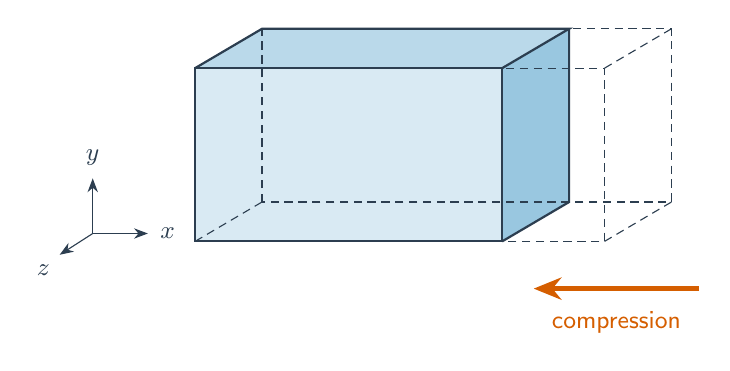
\begin{tikzpicture}[font=\sffamily, text=slate]
  % oblique depth vector
  \def\dxx{0.85} \def\dyy{0.50}
  \def\Lo{5.2}   % original length
  \def\Lc{3.9}   % compressed length
  \def\H{2.2}    % height

  % ---- compressed prism (solid, shaded) ----
  % right face
  \fill[oiblue!40] (\Lc,0) -- (\Lc+\dxx,\dyy) -- (\Lc+\dxx,\H+\dyy)
                   -- (\Lc,\H) -- cycle;
  % top face
  \fill[oiblue!27] (0,\H) -- (\Lc,\H) -- (\Lc+\dxx,\H+\dyy)
                   -- (\dxx,\H+\dyy) -- cycle;
  % front face
  \fill[oiblue!15] (0,0) rectangle (\Lc,\H);
  % visible edges
  \draw[solid edge] (0,0) rectangle (\Lc,\H);
  \draw[solid edge] (0,\H) -- (\dxx,\H+\dyy) -- (\Lc+\dxx,\H+\dyy)
                    -- (\Lc,\H);
  \draw[solid edge] (\Lc,0) -- (\Lc+\dxx,\dyy) -- (\Lc+\dxx,\H+\dyy);

  % ---- original prism (ghost, dashed; drawn last, never masked) ----
  % back face
  \draw[ghost] (\dxx,\dyy) rectangle ++(\Lo,\H);
  % connectors
  \draw[ghost] (0,0)     -- (\dxx,\dyy);
  \draw[ghost] (\Lo,0)   -- (\Lo+\dxx,\dyy);
  \draw[ghost] (\Lo,\H)  -- (\Lo+\dxx,\H+\dyy);
  \draw[ghost] (0,\H)    -- (\dxx,\H+\dyy);
  % front face
  \draw[ghost] (0,0) rectangle (\Lo,\H);

  % ---- compression arrow (underneath) ----
  \draw[force] (6.4, -0.6) -- (4.3, -0.6)
      node[midway, below=4pt, font=\sffamily\small, text=oivermil]
      {compression};

  % ---- coordinate triad (z out of the page) ----
  \begin{scope}[shift={(-1.3,0.1)}]
    \draw[axis] (0,0) -- (0.7,0)       node[right=1pt, font=\small] {$x$};
    \draw[axis] (0,0) -- (0,0.7)       node[above=1pt, font=\small] {$y$};
    \draw[axis] (0,0) -- (-0.42,-0.27) node[below left=0pt, font=\small] {$z$};
  \end{scope}
\end{tikzpicture}
\end{document}
